\chapter{Implementation}
  The fully implemented product has been derived by the guidelines received from Elizabeth Sklar, King's College London who guided the implementation of the report and provided a Server package that in turn is now the main communicator of information of the finished product. This product can be broken down into several components these being(For a better explanation please refer to figure 1):
  \begin{itemize}
    \item Simulation Environment - A composition of packages composed of: Server Control, Robot Control and Robot Simulation.
    \item Server - A package composed of communication protocol classes.
    \item Hider - Composed of classes responsible for server connection and Hiding the treasures.
    \item User - Composed of classes responsible for UI, server connection and Remote Robot Control.
  \end{itemize}

  In following sections of this report, a more broken down structure to provide insight into how each of these is achieved.

  \section{Simulation Environment}
    As stated before, the ROS stack is a combination of three packages. The Server control, Robot control and robot simulation. They interact with each other in exactly the way that was stated in the design with Server control connecting to the robot control that then sends commands to the robot simulation however a more precise definition will be given in the next sections.

    The implementation also makes use of launch files to reduce the number of terminals that have to run during the execution of the simulation environment. This is due to the fact that with just the launch files given in the ROS tutorials, the amount of windows that have to be open for executing the environment can increase quite exponentially with the number of robots and is in no way automatic.

    This launch file further lists the important packages that implement the simulation and exposes user to the outline of how the ROS environment operates with further explanation of packages outlined in next sections of the implementation chapter.

    \subsection{The Server Control}
      The Server control implementation is based around creating a serverToController package outside of the ROS simulation. This is done to ensure that a modular approach was taken and the server can be extracted and replaced if such a need occurs. It also takes advantage of publisher/subscriber method to implement a workaround Observer Design Pattern that allows two classes to work together using callback functions rather than the Observer fire() events and implementing extra interfaces. This in turn, creates a much simpler to work with environment where the communication between two classes is transparent and callback methods are limited in their simplicity. It also implements C++ threads to allow socket connectivity through clients thus allowing a C++ server to connect using TCP client to the Java Sever running on currently a local host machine.

      The server control also ensures that no commands that are irrelevant to the Robot controller are sent through. This includes commands like \%\%ack or \%\%ping that only need to be answered by the server control. This in turn creates a sieve for commands from the server with only useful ones going through.

    \subsection{The Robot Controller}
      The robot controller is inside the same package that the Server control is based in. This is mostly to ensure that while modularity is kept, the classes aren't spread out so far inside an environment that it would make it difficult to troubleshoot. Also since these two nodes have a ROS topic that is dedicated only to themselves, it makes sense that they would be stored inside the same environment.

      The controller is used inside the ROS environment to communicate between the server commands and the robots themselves that are simulated and switched on along the server control and the controller. This controller send information to robot\/move\_base\/goal to send the robot a goal command that they need to reached. It has pre-programmed room numbers in a form of two separate array for x and y coordinates with the array positions representing room numbers for simplicity. This means that to access room 0, the program will look values up from x[0] and y[0]. A separate class could have been created to hold various rooms however creating and referencing objects in ROS can be quite tricky. It requires editing the CMake files and linking libraries for ROS automatic compiler that sometimes can get a bit buggy with ROS only allowing a handful of commands from the original C++ compiler.

      This can be very well seen when in the server control package as well as in the robot controller where the thread development was done through pThread class that C++ implements. There were other options online that allowed the same type of thread creation however a limited number of allowed C++ classes in the ROS stack has made it very difficult throughout the project to search for the ones that are allowed.

      Robot controller uses threads to ensure that when the goal is sent, the variables inside the thread are kept and unchanged(like which room was selected or which robot is it as identifiers would have to be broken down causing higher resource usage) during the robot reaching its goal. Since the method has to wait until a single robot comes back with a command that says that the goal has been reached, a thread was the perfect choice for this approach. This approach allows scalability and publishing to tf prefix topics was chosen to ensure that as many robots as possible can be controlled through this package.

      Once the robot has reached its goal that the thread was waiting for, a command is issued that published to a topic shared by the controller and serverToController that the package picks up using subscribe, calls back a method and later on sends it to the server. With this approach, the environment is never blocked concurrency wise but also makes the controller responsible for only the task that is controlling the robots.

      Finally, it is important to mention that currently the GUI does not allow altering the goals. This can be done, however it is important to note that when two subsequent threads are created for the same robot, the previous thread will get canceled and a message regarding reaching goal failure will occur. This actually makes sense because the changed goal means that previous goal is not reached however if a GUI is created that takes into account failure of reaching goals and allows altering them midway, it could pose issues for the developer that decides to create their own UI. Whenever a goal is altered then, a developer will need to be aware that they will receive a goal failed message and the previous node will die out to preserve resources.

    \subsection{The Simulation Environment}
      The simulation environment runs on an indigo version of ROS setup in Ubuntu. Most of the code has been developed using the Ros Wiki tutorials and as such some packages are directed in such a way to follow the standard set out by the ROS system. The system fully allows for multiple robots to exist on one simulation of the environment and takes advantage of the launch files to do so.

      All of the code for the ROS simulation environment is actually held in 2 separate packages. One package is for the environment and another is an exportable package holding classes for filling out the GridLayer.

      GridLayer was a plugin developed to create extra layers inside the costmap that is responsible for avoidance of obstacles inside the ROS environment. It's main motivation was to allow for robots to be notified of each others presence on the map and build planners accordingly to situations that might require each robot to avoid another. At this point in time, the ROS environment has a significant input lag that doesn't update the map in time for the robot to take advantage of the newly filled out layer. Updating the map in real time is actually quite unresponsive with occasional updates leading to a conclusion that at the time frame allowed for this project, updating the Grid Layer would not be feasible as it would require to go into the ROS environment and modify the codebase. This in turn would require a tremendous amount of resources.

      This however is not an issue for an environment that operates in real world rather than simulation as in real world the robot would build up its costmaps based on sensor input data that it receives. So while the project is in its works with regards to simulation, in future works that bug will turn out to be non existent and won't cause concern for the researchers. With that information, the implementation moved further.

      The other main package for the simulation contains nodes responsible for robot movement. Information like odometry, mapping of the topics as well as pose publishers are all present there and they are all edited so that they allow for multiple robots to run simultaneously and all be launched from a single launch file. This was achieved by doing two things: passing parameters to the robots with a certain robot number as well as including a tf\_prefix for specific robot groups so that the packages would not have to be reinvented. Such approach provides functionality that allows unlimited amount of robots to be launched using a launch file with only one visualization tool required to represent them.

      There is however a small issue to be addressed here. While the nodes are designed to work with as many robots as possible, the launch files that allow for fake localization are not quite as diverse and don't allow for parsing parameters to them. This is a challenge that the project encountered when trying to simulate the robot using the same fake localization files. It was later realized that fake localization uses topic names and as such configurations that are switched on but don't have their fields altered to include robot number prefix fail and create error reports at the start of the simulation.

      To go about this issue, extra launch files had to be created as that was the only way other than distorting the codebase to include configurations at the grouping. While this solution could be simpler it proposes a solution that is a whole lot messier and more difficult to keep up with if extra robots were added to the simulation. A suggestion of creating a package that generates the launch files can be drawn. It would require one parameter that takes in the amount of robots and with that generates all the logic so that the main launch file is also generated and running it, consecutively runs the simulation with the amount of robots specified. It is an easy solution however it falls outside of the scope of the project with regards to the time frame given. It is however a consideration to be taken on if the project was to be improved on.

      \subsubsection{Mapping in ROS}
      Mapping is the building block around the Robot Operating system. It works by mapping topics to other topics to make sense of the data. In the figure below we can see how the current implementation maps topics for a single Robot.

          \begin{figure}[htp]
            \makebox{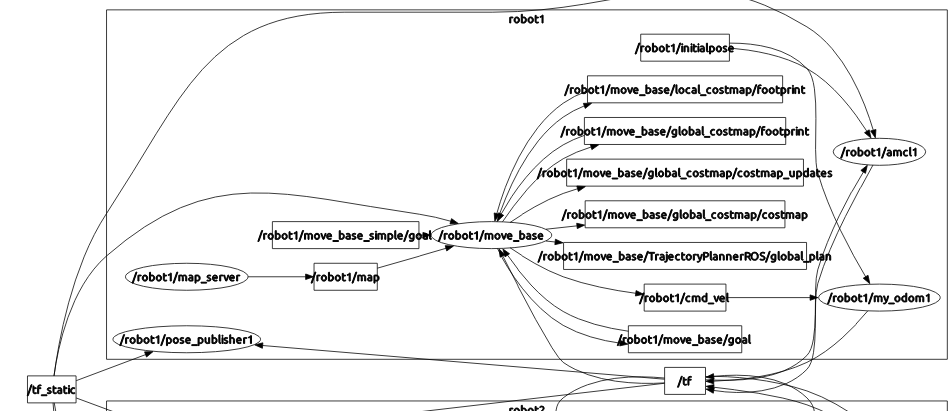
\includegraphics[width=1\hsize]{figures/ROSmapping.png}}
            \caption{Mapping of packages for a single robot.}
          \end{figure}

      This figure is only limited to topics that at the time of producing the graph were active. Several topics start to only publish at certain point like when a goal was reached so it goes to show how useful the launch files are and how many windows would otherwise had to be created to run all the topics separately.

      As previously stated ROS uses mapping to map certain topics to each other to be able to make sense of the data. Topics are generally nodes that publish any sort of data or can even be physical objects that map from one to another. This can for instance be mapping a robot hand to the body. This means that including a mapping graph gives a great deal of the implementation in the environment. The mapping graph however does not show which topics listen or publish data from and to each other and that's why in the previous figure, there is no connection between the goal node and the outside(not visible on this figure) controller node that would actually send data through about where the robot should go. Such graphs would be extremely complex and at larger levels unreadable.

      This figure then, was also included in the project to demonstrate the architecture behind how singular robots work inside the ROS environment. It lists every class developed in the Robot package along with those pre-build by ROS to aid in simulation. Perhaps the most important package inside the environment is the Odometry package that will be discussed further in the next section.

    \subsubsection{Odometry}
      Odometry is the use of data from sensors in robots to estimate their position in the environment. The location can never be exact as some things like slide or drag or friction when the robot is moving could slow it down causing a the estimation to go off if it doesn't take those into account and even then, the location will not be as accurate. In the simulation environment, this odometry can be considered to be very accurate and in the simulation package, odometry does very little in terms of robot estimation. This package in ROS, when ran is actually mostly used to collect velocity controls from the amcl that does the localization.

      AMCL is a probabilistic localization system for robots moving in 2D that implements a monte carlo localization approach through the use of particle filters. The science behind it is very complex and the implementation is done in ROS and available as a given package. As such it is unnecessary to further mention it than to explain that it is used for main planning using the map given and publishes velocities that the robots should take to ensure that it is in the correct position and that the amcl can follow its path.

      With this information, it is easy to infer that the odometry package for this project in ROS is responsible for accepting velocities and upgrading the robots pose by this estimation. Through that, it does follow the principle of holding the position but rather than the estimation mentioned in the definition, in the environment that is used as simulation this figure is much more precise.

      Odometry is also responsible for mapping of several topics and as such, it is one of the packages that is both a subscriber and a publisher. It subscribes to messages regarding velocities and publishes mapping required for the robot to move along the map and be visible to both the visualization software as well as amcl and move\_base that are responsible for implementing robot goals functionality. Some of these move\_base packages and amcl topics can be seen on figure 5.1.

      To make the odometry applicable to all the robots separately, there was a function implemented called getName that produces topic names based on the number received from the arguments. This simplistic approach allows for the same odometry node to be reproduced saving a lot of time with coding and compiling multiple odometries for each robot separately.

      For any future developers, it is important to note that Odometry that is present in the ROS Wiki pages at the time of writing the report does not implement any of the listening and publishing. It also moves the robot forward without any command given. There is even a lack of mapping the odometry to the robot which is not mentioned in the Wiki which for beginning developers might raise a lot concerns that their code is not working. This stalled the development of the environment by considerable amounts and with such a small community everything had to be worked out through trial and error.

      The next sections discuss in more detail how amcl and move\_base packages work for further understanding.

    \subsubsection{AMCL and move\_base packages}
      The amcl and move\_base packages are the packages that allow the robots to move through the plane in the current simulation environment. Without these, the robots would stand in place with no data. They connect the robot and odometry to the map and create obstacles based on the input data from the map. This in turn allows for maps to be created .png files and speeds up the process of rolling out new maps for the robots.

      They do however pose a certain difficulty when rolling out the robots. As previously stated these packages were not created to support multiple robots and they are implemented using yaml files that are static uncompiled interpreted files. This means that variable parsing is not allowed as it was with the odometry packages and separate files have to be created for separate robots. The solution to this was already discussed in previous sections.

      The move\_base package takes in five files in the current implementation all of which define the costmaps for each specific robot. This move\_base then creates the obstacles and allows the planning to be created for the robot and publishes cmd\_vel topics that were previously stated to be subscribed to by the odometry.

      This in turn creates defines the backbone for the robot environment with single robot environment explained in great detail. The next section outlines the how these packages together are taken to create a multi-robot platform.

    \subsubsection{Tf\_prefix and Multi-robot Functionality}
      It is important to note that tf\_prefix is considered deprecated in future releases of ROS due to developers not making good or any use of it with several packages starting off with the lack of support for tf\_prefix. However, it is also important to note that without it the project could not implement the multi-platform the way it did with a clean approach that allows to add robots using a simple checklist.

      The launch files in ROS take on a role of XML defined information sources for ROS to pull in and switch on nodes based on the information on them. This way rather than switching on topics like roscore and rviz, everything can be defined to be switched on automatically saving a lot of terminal windows being open. In this project, one launch file creates a two robot environment with server connections all in one terminal using only one command.

      This kind of approach using tf\_prefix allows for a list to exist that if followed to the letter will allow a developer to add a robot to the environment in an automatic way:
        \begin{itemize}
          \item Copy an existing groups XML code
          \item Increment all the arguments parsed by one
          \item Create separate local, global and common costmaps for this robot using the old ones and increment mappings by one.
          \item Direct move\_base parameters to these files
        \end{itemize}

      This short list allows for another robot to be created with ease. In the GUI all that has to happen is to increase the number of robots allowed to be selected in the source code and compile the code. This is to emphasize that the environment was created with customizability in mind. This section also summarizes in great detail the most important aspects of the implementation of the simulation environment. Further sections will discuss the challenges met along the way with implementing the simulation environment.

    \subsection{Challenges in simulation implementation}
      The implementation of this environment in 2D Ros was by far the longest process throughout this project. Due to ROS's continuous and rather violent growth a lot of Wiki's are outdated and the community tends to be very non responsive. A lot of the work that went into this had to be trial and error based with various packages working and not working through the development phases.

      Another note to make is that ROS implements its own version of a C++ compiler that does not contain all the packages that a regular user might wish to use especially when it comes to multi-threading. This became especially difficult to use when making plugins as referencing classes to each other turned out to be a very tedious and buggy process. Some plugins also turned out to spin(Ros uses spin to loop over topics and make callbacks based on each iteration) which made it impossible to subscribe directly to topics if that specific plugin was used. This made some of the development quite difficult especially the Grid Layer. Later on with testing it turned out that the Grid Layer couldn't process the information properly anyway which leads back to the point made about ROS's expanding growth and packages not being able to keep up. At the current moment ROS is an amazing architecture however at times one of its biggest challenges is that it makes it difficult for the developer to create clean readable code due to workarounds needed to push it to its full potential.

    \subsection{Final notes for Simulation Environment}
      A full implementation of the simulation environment runs using Rviz as a platform for testing whether the robots work. The navigation stack is fully implemented and accepts commands being taken in. The logging feature is switched on and ROS generally fills up on information quite fast so its absolutely essential that if used in the future, the developer should switch logging off unless they actually wish to troubleshoot. Otherwise ROS could overflow the drive quite fast after about 20-30 runs. Without logging these resources are well preserved and don't use up this much of the computers resources as no visualization software needs to be ran.

  \section{Server}
    While the server was fully implemented by  Sklar and Parsons\cite{technical}, it is the main tool that connects the environment and the GUI and with that, the commands and integration of this package into the system is important to discuss.

    The server can work on any operating system and will open up the Socket to computers connected in Local Area Network. If the computer enables connecting to it through the Internet using a dedicated IP, it would also be possible to host this server on a dedicated hosting machine that would then allow the environments to connect through the Internet and as such allow a much more flexible way using connections.

    This server accepts a big variety of commands to which explanations can be found in \cite{technical}. In this report however, only the commands that are used by the system will be discussed. These commands are:

      \begin{itemize}
        \item \textbf{\%\%setid} - When an application connects to the server it sets its id to receive messages from other applications.
        \item \textbf{\%\%ping} - Command sent by the server to applications to ensure that they are still connected.
        \item \textbf{\%\%pong} - Response to the ping command to confirm connection.
        \item \textbf{\%\%send} - Generic message send from application to application.
        \item \textbf{\%\%goto} - Command sent from UI to the simulation environment to move a robot to a place on the map.
        \item \textbf{\%\%found} - Command sent from UI to the Game master(In this implementation from hider to the UI) about information about location and characteristics of the server.
        \item \textbf{\%\%snap} - Command sent from the UI to the Hider to ask for an image of the treasure.
        \item \textbf{\%\%image} - Command sent from the Hider to the UI informing about the file which stores the specific treasure.
      \end{itemize}

    This outlines the commands used by both the UI and the simulation environment used in the current implementation. In the future sections, a discussion is created based on the conventions set by the technical description in \cite{technical} as well as an explanation of how each specific command is used in the implementation of the system.

    \subsection{Conventions}
      The server outlines some specific conventions by which the applications should connect to the server. These are by no way enforced however for ease of debugging they have been implemented in this system. This was also done to standardize how the system behaves. The name convention of apps connecting to the server are as follows:

        \begin{itemize}
          \item \textbf{SimR}: The simulation environment.
          \item \textbf{TabUI}: The GUI on the user side.
          \item \textbf{Hider}: The treasure knowledge base that holds information on which treasures are present in specific places.
          \item \textbf{Server}: The server running in Java.
        \end{itemize}

      It is also important to note that these names allow for generation of messages at source code level without having to create external files for what's the name of specific components in the system. Changing those at the current level of implementation would cause the system to malfunction and not deliver messages unless recompiled with changed names. For flexibility in the future, it could be possible to pass these as parameters in the main execution at terminal level or include external files.

      It is also important to note that the port used by the socket has been selected to be 6009. This is to inform that the server needs to be switched on with this specific port otherwise the applications won't be able to switch on properly. This port has been selected due to its availability and on most operating systems it is not used by any software so it is a safe option. On top of that it has been confirmed to guarantee complete data transfer on TCP level. It is only used be x11 windows server which generally does not use it anyway. With regards to threat it is not a targeted port so it keeps system security optimal. For information on this port please refer to \cite{port6009}.

    \subsubsection{Use of specific commands}
      This section outlines specific flows of data throughout the application to give a better image of how the server is being used. Each of those commands plays a specific role and there a demonstration of flow for specific situations is explained.

      \subsubsection{Connecting to the server}
        The connection to the server is fairly simple for Java while a bit more tricky for the C++. When Java connects it immediately sends a request to the server to set the id of the application(Using the \%\%setid command). It then receives an \%\%ack command that can be ignored and simply confirms that the id has been set by the server. If the socket doesn't exist, the application terminates. If the application receives a shutdown command it will still work for demonstrative purposes of the application but this only happens if the application was switched off and didn't give server time to clean out the old id that will not respond to the next ping request.

        This works in a similar manner to C++ however with C++, there is almost no way to deal with the server not connecting and the C++ will start to complain about lack of existence of to the server filling up a big chunk of the ROS logging utility and take up drive space. The only way is to set a timeout to connecting to the server however that will also slow down the flow of information so before switching the simulation environment, it is best to start up the server or to comment out the node packages responsible for connecting to the server in case of testing the environment.

      \subsubsection{Sending a robot to specific location}
        Normally it is possible to send the robot to any location using x and y coordinates but in the current implementation of the system these are hard coded at the simulation environment. This means that rather than using the standard goto command that accepts x and y coordinates, the x and y coordinates are both set to the room number the robot is finished. It would be better to use only one argument for the room number but at this point in time the server is very specific about the number of arguments it receives. This then is passed through the server to the simulation environment and the robot is sent traveling to a specific room.

      \subsubsection{Robot reaching the goal}
        When a robot reaches its goal, the environment sends a generic message in the form of "robotNo;roomNo". This message is very easy to understand and when a client receives a message of type send with these arguments it updates the map and starts initializing the dialogue for taking the treasure.

      \subsubsection{Asking about the treasure}
        To receive the first information about the treasure the client sends a quick message to the Hider class and waits for a response before showing user the dialogue. This request is sent as soon as the UI receives the news of robot reaching its goal for efficiency. This message is a generic send message sent to the hider with a room number as an argument. In the hider this message is easily decrypted and a reply is sent using a found type message that contains the details about the treasure.

    \subsection{Final notes about the server}
      The server is a great piece of work that saved a lot of time during the implementation of the entire system. With it the environment only has to connect, set an id and the messages are being send back and forth without a problem. There are small issues like the time it can take to clean up old clients to reconnect again but that would consume resources on a computer and would not really affect the working system as much. It is only useful for testing.

      Another big note to add is that the server at the time of implementation notify a client of a message being sent successfully or failing to do so because some other client disconnected. This means that troubleshooting is more difficult as this type of lack of responses leads to having to develop more generic messages that could make the system more complex and messages have to be generated at both sides rather than simply filtered.

  \section{Hider}
    The hider is a package responsible for taking in a file in a template format and converting the information stored inside it to produce a list of String arrays that can later be used by other packages for information on Picture information, treasure outlines etc.

    Normally this data would be acquired from the robot with the hider only hiding the specific treasures inside a map and would be the only other class(or even a robot carrying out the job) that would place the treasures in the arena and later on hold identification details that can be retrieved from it by commands however all its responses are sent to the TabUI even if they could potentially be from somewhere else. This is specifically to ensure that no one can listen to the data packages and with that create a safer environment.

    The before mentioned template file holds information in the following manner: the first line is just a number with a number of rooms while the next lines are written as "Colour, footprint, score for the treasure, what the treasure actually is, image file that holds the treasure data". This was done to allow as much flexibility as possible with regards to adding extra treasures and add different levels of ambiguity. The User template for treasure information holds the same data without the information of the image file. This way, the users cant peak at source code to find it.

    To make the game more interesting and stop people from cheating after a new game, as stated previously, the Hider generates a random HashMap of treasures and hides them throughout the map across the number of rooms specified so it is possible that some maps will score more points and be more ambiguous but this can be adjusted by adjusting the values and ambiguity of the the treasures themselves.

    The Hider does not boast any sort of GUI as the template is simple enough to edit using any editor of choice. With the edited template, when the system is restarted, the Hider will read in a template like it would with previous examples.

    Similarly to the User package, the Hider had to implement an Observer design pattern with its own dedicated client socket connection to listen to the commands that come in. The Hider class is above the server class and as such the Server should only be able to accept commands coming from the Hider rather than the other way around. With that in mind, an Observer pattern seemed to be the best choice.

  \section{User}
    The User section is an outline to how the TabUI environment works and how the data is produced. It will shed more light onto the calculation of the cost for the path travel for the robot and how that path is calculated as well as present a finished product outlining how the game works using a series of screen shots to support it.

    As stated in the design section, the User UI was developed using Java Swing interface to save as much time as possible before rolling out a fully implemented product. This product consists of various classes which will be outlined in the previous sections however at the heart of the program is the GuiUser class that is responsible for handling the logic of the program as well as the GUI. It consists of various methods and takes advantage of classes that can be considered below it when thinking of the system hierarchy.

    The classes implemented for this package are: GUI frame, Dialogue class, Robot class, RobotRenderer class, Command Object class and Connector class. Each of these classes will be outlined in more detail with the ones that use the least dependencies being the first to later build up how the next classes use these for a better explanation.

    \subsection{The Dialogue class}
      The dialogue class is the main focus of this report. It holds information on costs for going to each room on the map from another as well as providing customizability to the report. This class in itself provides the GUI with a tremendous amount of functionality.

      The reason why the costs of reaching a certain path are calculated here is because ROS robots do not follow the path directly and in a simulated environment it is impossible to actually develop a function that could predict how long the robot will take to get from one room to another especially with this many variables. This leads to a conclusion that data collection will have to occur in order to start producing cost prices. This was achieved by timing the robot on its way to each room in the arena from the other room to create average times for each of these. This was also achieved using the GUI for testing purposes to ensure that the times coincided with when the GUI receives a full response. With the fully collected data, an adjacency matrix was created with y coordinates being "from" and x coordinates being the "to" nodes while the element would be the cost of going to the next path. This adjacency matrix was then stored inside a separate file that holds information separates by lines with spaces indicating a break between nodes. This kind of approach allows for easy reads from the Dialogue framework. It can be argued that to secure these files, it would be a good idea to encrypt this information when it is saved in a file but for the purposes of this project keeping it in an easily editable file seems a preferred choice. The dialogue class is also responsible for providing the UI with the costs to minimize reinventing the wheel of reading in the files or holding multiple instances of the cost map.

      This calculation was then used to produce suggestion to the user to ensure that when they click the "Don't know" button they will be presented with a room suggestion. The reasoning for calculating the best suggestion could be considered to be the closest room however the robots will all follow to closest rooms and both will cover the same amount of distances. To alleviate this issue an algorithm was devised for calculating Hamiltonian Shortest paths. This algorithm calculates all the permutation of paths for unvisited rooms which is supplied by the GUI, picks the cheapest cost permutation and returns the next room on that permuted path to the user. A pseudo code for this algorithm then is:\\
      \textbf{Optimal next room selection}\\
      \emph{
        \textbf{Input: } Current room, Unvisited room list\\
        \textbf{Output: } Optimal room suggestion\\
        1. Calculate all the permutations of unvisited rooms and append room at the beginning of each.\\
        2. Calculate the cost for each of these paths.\\
        3. Find a path with minimum cost.\\
        4. Return the first next room on that path.\\
      }

      This algorithm follows a complete approach to returning the most optimal route a user could take throughout the map. Since the problem of such paths is considered NP-Hard the solution to it runs in O(n!) for listing all the possible permutations and as such is not a very efficient algorithm. This is not an issue in the current implementation of the game(and probably future ones) as the number of rooms is probably never going to exceed 10-12 which wouldn't slow down the application at the slightest. By a slight tweak to it, it can be deduced that using the current adjacency matrix and starting at the corridor, the optimal cost of traveling through the map without taking pictures would be 130 while the maximum is 182. This means that one robot has no chance of visiting all the rooms and more robots are necessary for this particular scenario. This is good as it forces the user to use multi robot environments and gives good reason as to why developing multi robot frameworks is necessary.

      The next task that the dialogue is responsible for is handling the conversation. In this situation, two modes are available. One for selecting specific rooms and the other for the user not being sure. This is achieved by another template with reserved keywords so that researchers don't have to dabble in the code to get their results. This template is held inside the "dialogueText" file and contains a list of questions. The first line in this file is for reference. This line can be used to describe the file. The lines following this one are questions that the user is going to get asked consecutively to reach a consensus. If no consensus is reached the dialogue restarts and waits for questions to be pulled in again. The reserved words in this scenario are £cost£ and £room£. The class is going to replace those with actual values when the GUI requests a question and will keep an unformatted version throughout.

      To create a more robust environment that can be edited without replacing dialogue classes in the GUI section, the dialogue could be taken outside of the GUI frame and implemented as a separate class that connects to the Server and replies to specific commands however for the purposes of performance it was kept inside the GUI frame to allow easy iterator style pattern for retrieval of questions. Otherwise, a lot of generic messaging would have to be implemented.

    \subsection{Robot class}
      The robot class is responsible for holding information about the robot that the GUI believes to be true. It holds various variables that tell the GUI about its location, whether or not it is traveling, what's the cost for the path that it has undertaken, the number of the robot and its remaining energy. All robots start at 100\% capacity and go down from there. The robot blocks itself and is not able to move or accept commands when it reaches 0\% energy level.

      There was not enough time to stop the robot from going to rooms if it has less energy than the room it wants to reach however even if it goes to visit that room, it is not going to be able to take a picture or move anywhere else from there so in that essence, it stops people from being able to reach cheat the game by leaving the last room furthest away to then visit and take advantage of this little bug.

    \subsection{Robot renderer class}
      This class is responsible for taking in the robot information and display it as singular cells on the side panel. It uses most of the robots getter commands to inform the user that the robot is traveling, what room it is in and show a progress bar when the robot moves. It is changed when the GUI calls a fire command to this table and with that allows travel between spaces. The main task of this class is in aesthetics but it is important to mention it here for a reference point of where to look for data. This class does not manipulate any robot or GUI logic manipulation and is in no way connected to the server.

    \subsection{Command Object class}
      This class is responsible for passing commands from the server to the GUI but is also implemented by the Hider class to serve the same purpose. When a command comes to the server it changes a value in this command and a value changed is fired. This data can then be further processed by the GUI.

    \subsection{Connector class}
      The connectors aim is to connect the GUI to the server(Same separate version is used by the Hider class). It is a client package that does not alter any game logic and its main task is to keep the connection to the server up as well as receive and send commands to the GUI.

      The GUI holds direct reference to this class and is therefore above it while the server itself holds reference only to the CommandObject that the GUI has. This is to prevent access to more information than is necessary by it and to keep the logic only in the GUI.

      Another purpose for the connector class is command filtering. There are various commands coming from the server. There are ping messages that the connector replies to automatically without passing it further to the UI, there are commands like send, image or snap that it accepts and passes it on and finally there is an acknowledge command that it does nothing with at this point in the project. This last command is an acknowledgment that the server has successfully received a message from the Server and as such this confirmation is only necessary for the Server. In Java environment, if the server breaks connection, the client sockets will switch off automatically so checking the connection with the server is unnecessary. Other commands are disposed off and are not passed any further down the line to ensure that the GUI is not burdened with junk data.

    \subsection{GuiUser class}
      The GUI is the heart of the User side of the application. It is responsible for directing the logic of the game as it is set out in this scenario and is the longest block of code in the application. This is because the GUI and the way it runs the game should be centralized to minimize extra files that might confuse someone that wants to implement their own logic or edit the current one. It follows the logic set by the treasure hunt game outlined in \cite{Elizabeth} and allows for almost all of the functionality set out by the specification chapter.

      The complete product can be seen in the figure below:

      \begin{figure}[htp]
        \makebox{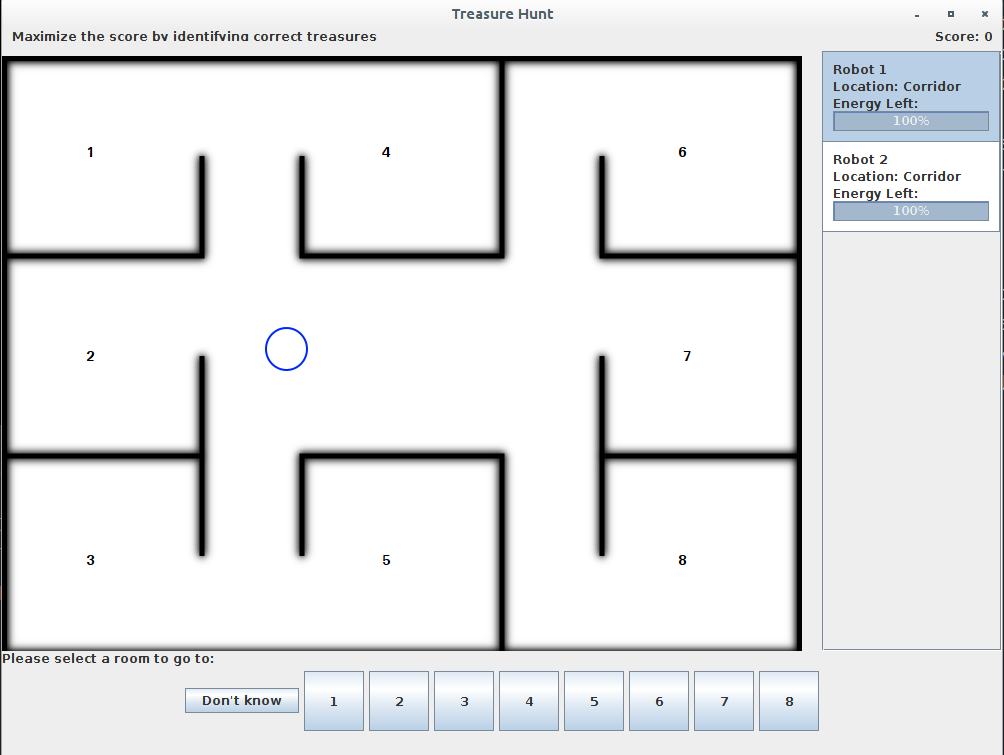
\includegraphics[width=1\hsize]{figures/finished.png}}
        \caption{Finished GUI.}
      \end{figure}

      The aim was to create a GUI that is as intuitive as possible. With this one, the user has the option to do everything in the game in one window and with such GUI design it is extremely easy to push it to an android tablet or anything else to make it more convenient to use as the entire flow of the application uses buttons to communicate with the user.

      It is important to note that at this time of the project, since the robot is simulated, that features that the robot normally would be allowed to make are impossible here hence the environment was created to simulate things like taking pictures or sensing the treasures color and footprint. As such this is done by the Hider environment holding the footprints at room locations as well as file names for the images held inside the GUI class.

      Apart from that, as stated in the previous sections, GUI is the top class that holds references to all the other classes to present the GUI and handle the game logic. This type of hierarchy creates a simple and easy to follow architecture for both debugging and developing the environment. Wherever possible adequate variable names were used as well as minimal functions to provide code readability. More could have been done with regards to that however it is important to stress the short time frame given for a one person to develop such a complex system.

      The next section outlines the basic flow of the application with GUI figures for references about how the application makes decisions.

    \subsection{Flow of the application}
      The flow of application is important to outline in order to fully present the product. After discussing each implemented class and how they interact it is important to present a fully working product and how each interaction is created.

      The startup of the application requires the packages to be ran as follows:
        \begin{itemize}
          \item Start up the server with the port 6009(other ports are hard coded)
          \item Start up the simulation environment using the launch file provided.
          \item Start up the Hider class
          \item Start up the GUI
        \end{itemize}
      At this point the software is ready and the user is presented with the following dialogue asking the user how many robots it wants to use:

      \begin{figure}[htp]
        \centering
        \makebox{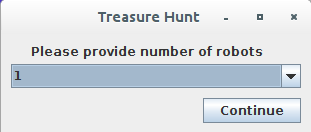
\includegraphics[width=0.4\hsize]{figures/App1.png}}
        \caption{Finished GUI.}
      \end{figure}

      This command is only used for the set up of the GUI. For simplicity reasons, the Simulation environment starts with 2 robots at the start however in the future functionality for starting the ROS stack could be created that creates Robots based on the command sent to it by the server. The amount of robots running at the ROS stack does not however, affect the functionality of the GUI and will work correctly with different amounts of robots set up at the GUI as long as both environments hold the same possible number of robots. In the current implementation 2 robots are set up to be the maximum however it will not be a problem to increase them as that is a single variable in the GUI and a matter of adding a robot group in the ROS launch file.

      After selecting two we are presented with the same image that can be witnessed at the figure 5.2. This figure shows the GUI when both robots are idle in the corridor. The map inside shows only one circle for the robot that is created. Drawing AWT map with robot positions updated showing all of them would be too time consuming for the purposes of this system and would take time off from developing the essential features. It would also consume quite a bit of resources with the increasing amount of robots being used. Currently there are 9 map images that represent where each robot is on the map. The objective of the game is to identify as much treasures as possible by either the footprint or by taking the picture of the treasure if the features are presented in a too ambiguous manner to be able to decide. After clicking the room, a dialogue is initialized informing the user of the cost to get to a certain room. As stated previously, this information is held by the dialogue interface from the average times it took the robot to get there.

      \begin{figure}[htp]
        \centering
        \makebox{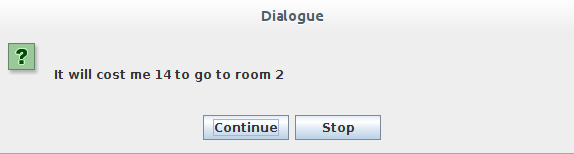
\includegraphics[width=0.4\hsize]{figures/App2.png}}
        \caption{Dialogue between robot and user initialized}
      \end{figure}

      After selecting the room to which the user wants to go to the dialogue is initialized. If at any point the user clicks the stop function the consensus variable will be set to false and the message to send the robot to the room will not be ran. This is to ensure that the consensus is always reached. When the consensus is reached the robot is set to the traveling state.

      \begin{figure}[htp]
        \centering
        \makebox{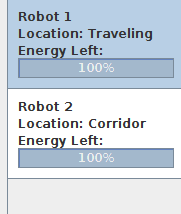
\includegraphics[width=0.3\hsize]{figures/App3.png}}
        \caption{Updated view of robot traveling.}
      \end{figure}

      Also the room that the robot is going to is marked as visited so when another robot is selected they cannot go there. This sort of functionality allows for making sure the user doesn't have to keep track of where each robot already went which can lead to potential loss of energy as well as the game dragging forever. The robot should only visit a room once and as such this functionality is developed using this approach.

      \begin{figure}[htp]
        \centering
        \makebox{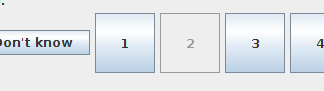
\includegraphics[width=0.4\hsize]{figures/App4.png}}
        \caption{Room no longer able to be visited.}
      \end{figure}

      After a while when a robot reaches a room at the environment stack side, the message is passed through the server to the Connector which informs the GUI of a new commands coming in. When this command is processed the GUI asks the Hider about the information about the treasure and waits for its response, when it comes in, the prompt is given to the user. It important to note at this point in time that if the Hider is switched on, the game functionality is forfeited for the robot to move around the rooms but not see any messages regarding the treasures and identifying those.

      \begin{figure}[htp]
        \centering
        \makebox{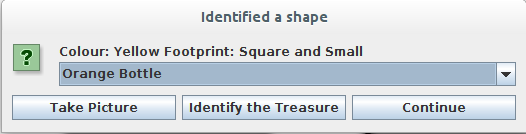
\includegraphics[width=0.4\hsize]{figures/App5.png}}
        \caption{Prompt with color and footprint of the treasure in a room.}
      \end{figure}

      This prompt allows the user to forfeit the treasure, take a picture of it or identify it. If the use forfeits the treasure by clicking continue they are taken back to the GUI and are able to continue the game. There are two moments at which the user is able to identify the treasure with this prompt being the first. When a user clicks Take Picture a command is sent to the Hider class that then responds with what image to show to the user. As stated before this is done to ensure that users don't get access to what treasures they are seeing.

      \begin{figure}[htp]
        \centering
        \makebox{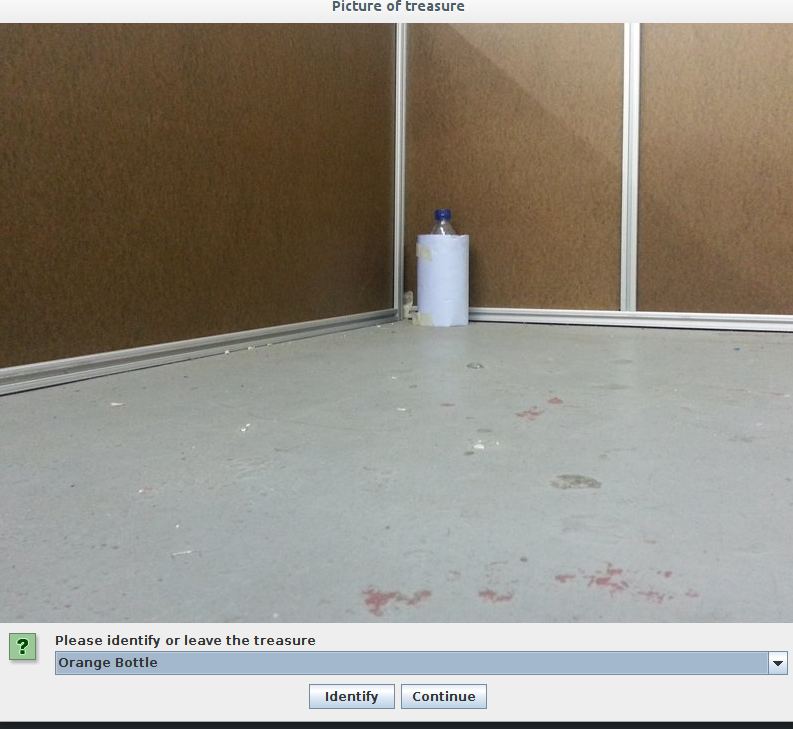
\includegraphics[width=0.4\hsize]{figures/App6.png}}
        \caption{Picture taking functionality.}
      \end{figure}

      After a picture was taken the user has two remaining options. To identify the treasure using a simple dropdown list or forfeit it if they feel like they can't make the decision and don't want to lose points. At this point if an identification is made, the GUI informs the Hider of the identification and receives a result about whether or not the treasure was correctly identified.

      \begin{figure}[htp]
        \centering
        \makebox{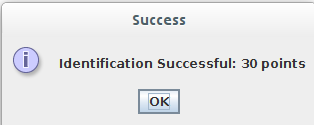
\includegraphics[width=0.4\hsize]{figures/App7.png}}
        \caption{Identification prompt}
      \end{figure}

      This message is just for information for the user to know what is going on and whether or not they succeeded in identifying the treasure. From this point on if there are no other dialogs in the Swing queue from other robots the user returns to the main screen and their score is updated based on the identification. They can continue to play the game until both robots run out of energy or all rooms get visited at which point the GUI informs them of the total score.

      \begin{figure}[htp]
        \centering
        \makebox{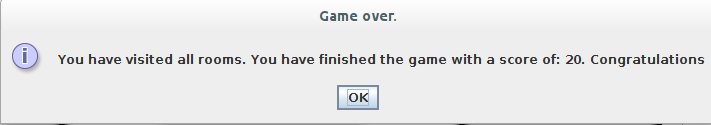
\includegraphics[width=0.6\hsize]{figures/App8.png}}
        \caption{Game finished prompt.}
      \end{figure}

      This final message notifies the user that their game has finished. They are notified of the score and after clicking OK the game terminates so it can be restarted by the next or the same user. Restarting the game won't load the old score nor won't it allow for the user to memorize maps as treasures are displaced randomly around the rooms with no probabilities for either treasure to be more favorable to be in one room to the other. For reference this kind of approach fully implements the logic outlined in the design section with both how the GUI is set out as well as the logic for the treasure hunt game.

      This summarizes the implementation outline of the project. Further chapters will test the system against the specification outlined in the beginning of the report as well as evaluate on the challenges encountered during the project and how they were overcome.